%% ----------------------------------------------------------------
%% EJEMPLO DE ARTÍCULO CIENTÍFICO EN FORMATO "AJCEAM"
%% Basado en la plantilla ajceam-class
%% ----------------------------------------------------------------
\documentclass{ajceam-class}   % Modo por defecto de 2 columnas

% -----------------------------------------------------------------
% Datos del Artículo
\title{Artículo 1: Redes bayesianas multinomiales}
\titulo{(Versión en Español)}

\author[1]{A01612830 Yoseba Michel Mireles Ahumada}
\author[2]{A01741659 Pedro Manuel Montes Valle}
\author[3]{A01741944 Santiago Pérez Mendoza}
\affil[1]{Tecnológico de Monterrey, Campus Guadalajara}

% Datos para cabecera y pie de página
\thisnumber{31}
\thismonth{Agosto}
\thisyear{2025}

% -----------------------------------------------------------------
% Resumen y palabras clave en Español
\abstract{
  Este estudio implementa redes bayesianas multinomiales para el análisis de patrones de movilidad urbana en la Ciudad de México utilizando la Encuesta Origen Destino en Hogares de la Zona Metropolitana del Valle de México (EOD) 2017. Se utilizó Hill Climbing como algoritmo de aprendizaje estructural, se modelaron relaciones entre variables demográficas, socioeconómicas y de comportamiento de transporte.
  Se abordaron cuatro escenarios durante el análisis: duración de viajes por estrato socioeconómico, gasto diferencial por género y edad, uso de transporte privado en adultos mayores, y comparación modal de tiempos de viaje. Se obtuvieron resultados los cuales evidenciaron diferencias significativas: 82.1\% de jóvenes en estratos bajos realizan viajes menores a 30 minutos, mujeres jóvenes gastan 15.3\% más que adultas, 57.4\% de mujeres mayores usan automóvil privado, y penalización temporal del 82\% para usuarios de transporte público en estratos bajos. Estos hallazgos revelan barreras sistemáticas de accesibilidad y eficiencia en el sistema de transporte, proporcionando evidencia para fines políticos. El estudio demuestra la efectividad de las redes bayesianas como una herramienta poderosa para el análisis de sistemas urbanos complejos.
}
\keywords{redes bayesianas multinomiales, movilidad urbana, aprendizaje estructural, inferencia probabilística, transporte público, Encuesta Origen-Destino, Ciudad de México}


% -----------------------------------------------------------------
\begin{document}
\maketitle
\thispagestyle{fancy}

% -----------------------------------------------------------------
\section{Introducción}
\firstword{L}{a movilidad} urbana constituye un sistema complejo caracterizado por interacciones entre factores demográficos, socioeconómicos y espaciales. La Zona Metropolitana del Valle de México (ZMVM), con 21.8 millones de habitantes, genera diariamente 34.6 millones de viajes \cite{INEGI2020}, presentando desafíos significativos para la planificación del transporte urbano. El análisis cuantitativo de estos patrones requiere metodologías capaces de modelar dependencias no lineales y relaciones probabilísticas entre múltiples variables categóricas.

Las redes bayesianas multinomiales proporcionan un marco matemático para el análisis de sistemas complejos con variables discretas. Estas estructuras probabilísticas, fundamentadas en la teoría de grafos acíclicos dirigidos (DAGs), permiten la factorización de distribuciones conjuntas de alta dimensionalidad mediante el principio de independencia condicional \cite{Pearl2009,KollerFriedman2009}.

\subsection{Marco teórico}
Una red bayesiana $\mathcal{B} = (\mathcal{G}, \Theta)$ consiste en un grafo acíclico dirigido $\mathcal{G} = (V, E)$ y un conjunto de parámetros $\Theta$ que especifican las distribuciones de probabilidad condicional \cite{ScutariDenis2021}. La distribución conjunta se factoriza como:
\begin{equation}
P(X_1, ..., X_n) = \prod_{i=1}^{n} P(X_i | Pa(X_i))
\label{eq:bayes_factor}
\end{equation}

El aprendizaje de estructura mediante el algoritmo Hill Climbing optimiza criterios de información (AIC, BIC) para identificar el DAG óptimo. La significancia estadística de las relaciones de dependencia se evalúa mediante pruebas de independencia condicional basadas en la estadística $G^2$ o $\chi^2$. \cite{ScutariDenis2021}

\subsection{Planteamiento del problema}
El presente estudio aborda cuatro interrogantes específicas sobre patrones de movilidad en la ZMVM:
\begin{enumerate}
    \item Probabilidad de duración de viajes superiores a 30 minutos en población joven de estrato socioeconómico bajo.
    \item Análisis comparativo del gasto en transporte entre mujeres adultas con destino laboral y mujeres jóvenes con destino hogar.
    \item Probabilidad de uso de transporte privado en días laborables para mujeres de 60-80 años.
    \item Comparación de tiempos de viaje en transporte público versus automóvil para estratos bajos.
\end{enumerate}

\subsection{Objetivos}
El objetivo principal consiste en el desarrollo de modelos de redes bayesianas multinomiales para el análisis de patrones de movilidad urbana utilizando datos de la Encuesta Origen-Destino 2017. Los objetivos específicos incluyen: (i) aplicar algoritmos de aprendizaje estructural para identificar dependencias entre variables; (ii) implementar técnicas de inferencia probabilística para responder las interrogantes planteadas; (iii) validar los modelos mediante criterios estadísticos; (iv) generar evidencia cuantitativa para informar políticas públicas de transporte.

% -----------------------------------------------------------------
\section{Metodología}

Este apartado se basa en el uso de \textbf{redes bayesianas multinomiales} para analizar los patrones de movilidad urbana a partir de datos de la encuesta Origen-Destino.

\subsection{Redes Bayesianas}
Las redes bayesianas ($\mathcal{B} = (\mathcal{G}, \Theta)$) están compuestas por: 
\begin{itemize}
    \item Grafos acíclicos dirigidos (DAG) $\mathcal{G} = (V, E)$, donde V se refiere a las variables aleatorias y las aristas de los nodos, mientras que E describe las relaciones de dependencia.
    \item Un conjunto de parametros $\Theta$ las cuales especifican las distribuciones de probabilidad condicional acosiadas a cada nodo.
\end{itemize}

La distribución conjunta de todas las variables se factoriza como:
\begin{equation}
P(X_1, ..., X_n) = \prod_{i=1}^{n} P(X_i | Pa(X_i))
\label{eq:bayes_factor}
\end{equation}

donde Pa($X_i$) indica los nodos padre del nodo $X_i$. Para variables categóricas, estas distribuciones condicionales siguen una multinomial cuyos parámetros se estiman con la ecuación de máxima verosimilitud. \cite{CIMAT} \cite{html_M1}\cite{html_Prob}

\subsection{Aprendizaje de la Estructura: Hill Climbing}
El algoritmo de Hill Climbing se aplica para determinar la estructura óptima; este algoritmo consiste en una búsqueda heurística la cual modifica el grafo iterativamente hasta optimizar los parámetros de información AIC (Criterio de Información de Akaike) o BIC (Criterio de Información Bayesiano) las cuales se expresan de la siguiente forma \cite{html_Prob} \cite{CIMAT2}: \\
\\
Hill Climbing:
\begin{equation}
G = arg max_G\,\,Score(G|D)
\label{eq:Hill Climbing}
\end{equation}

 \begin{itemize}
     \item Donde Score es una métrica basada en la verosimilitud y D el conjuto de datos.
 \end{itemize}
\\
BIC:
\begin{equation}
BIC = log[\hat{P}(nodos)]-\frac{d}{2}log(n)
\label{eq:BIC}
\end{equation}
\\
AIC:
\begin{equation}
AIC = log[\hat{P}(nodos)]-d
\label{eq:AIC}
\end{equation}


 \begin{itemize}
     \item $\hat{P}(nodos)$ es la probabilidad estimada global de los datos
     \item $d$ es el número total de parámetros de la red.
     \item $n$ es el número de observaciones.
 \end{itemize}


\subsection{Probabilidad condicional}
La probabilidad condicional es la base del razonamiento en redes bayesianas: 

\begin{equation}
P(A|B) = \frac{P(A\cap B)}{P(B)}
\label{eq:Prob-C}
\end{equation}

Esto permite el conocimiento sobre un evento A dado que está condicionado por evidencia B.\cite{html_Prob}

\section{Aplicación}
\subsection{Consultas en Redes Bayesianas}
Sobre las redes ajustadas se realizaron consultas probabilísticas mediante muestreos (cpquery) por ejemplo: 
$$P((T2 - T1)>30\, |\, (E=1 \& A<18))$$

\subsection{Implementacion de Redes Bayesianas:}

El algoritmo que utilizamos fue el de Hill Climbing para la estructura de la red, con este optimizamos el criterio BIC con el que posteriormente realizamos un gráfico acíclico dirigido o DAG con el que pudimos modelar las dependencias entre las variables que seleccionamos.

\subsection{Resultados:}

Analizamos 4 diferentes escenarios y nos dieron los siguientes resultados;\\


1.	Calculamos la probabilidad de que un viaje dure mas de 30 minutos dad que la persona es un joven del estrato bajo, El resultado que obtuvimos fue que con una probabilidad del 82\% es mas probable que el viaje dure menos de los 30 minutos. La función de probabilidad que utilizamos para este ejercicio fue la siguiente:

$$P((T2 - T1)>30\, |\, (E=1 \& A<18))$$
Donde:\\
T2 = Hora en que terminó\\
E = estrato\\
A = edad\\
T1 = Hora en que empezó\\

\begin{figure}[h]
\centering
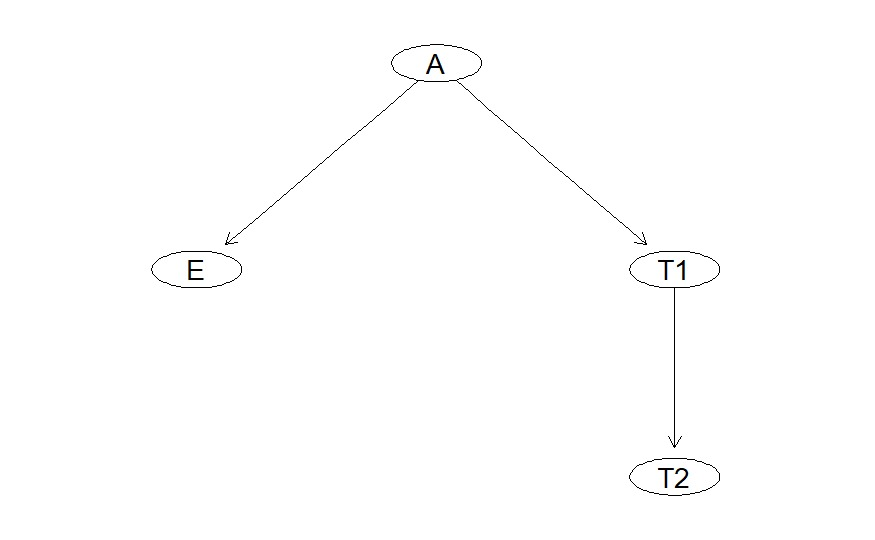
\includegraphics[width=0.45\textwidth]{img/dag1.jpeg}
\caption{DAG 1 - Red bayesiana para análisis de duración de viajes en población joven de estrato bajo}
\label{fig:dag1}
\end{figure}

2.	Para nuestro segundo escenario calculamos ¿Quién gasta más en transporte, las personas adultas que son mujeres y van a sus trabajos? ¿O las mujeres jóvenes que van a sus hogares? En este caso no se utilizaron del todo funciones de probabilidad si no que calculamos los promedios de gastos para cada edad y las comparamos para saber cual de estos grupos gastaban más en promedio, para esto utilizamos cpdist() para poder generar muestras condicionales. Obtuvimos como resultado que en promedio gastan más las personas jóvenes que van a sus hogares. Las funciones utilizadas fueron las siguientes:
$$E(G \,|\, S = mujer, A >= 18, D = trabajo)$$
$$E(G \,|\, S = mujer, A < 18, D = hogar)$$

Donde:\\
G = Gasto total\\
S = Sexo\\
A = edad\\
D = destino\\

\begin{figure}[h]
\centering
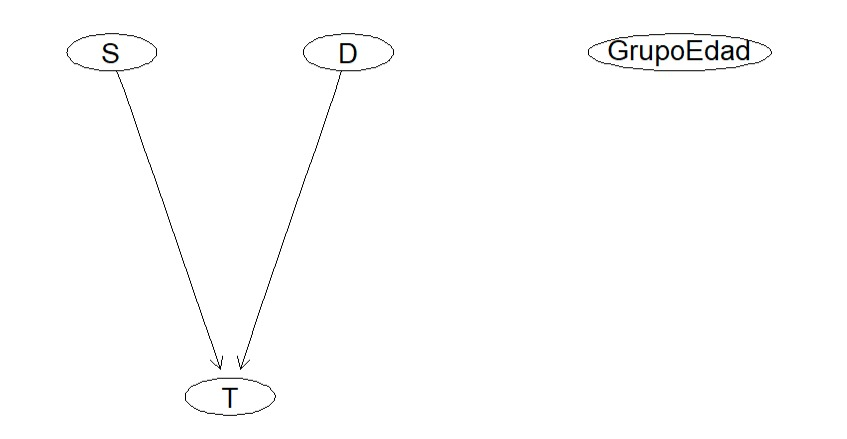
\includegraphics[width=0.45\textwidth]{img/dag2.jpeg}
\caption{DAG 2 - Red bayesiana para comparación de gastos en transporte entre grupos demográficos}
\label{fig:dag2}
\end{figure}

3.	A su vez calculamos ¿Qué tan probable es que una persona viaje entre semana con un transporte privado dado que sea una mujer entre 60 y 80 años? Obtuvimos como resultado que hay una probabilidad del 57% de que utilicen un transporte privado. La función de probabilidad fue la siguiente: 

$$P(M = auto\, |\,S = mujer, 60<= A <= 80, DL = 1)$$

Donde:\\
M = Modo de transporte\\
S = Sexo\\
A = edad\\
DL = Dia laboral (si(1) o no(0))\\

\begin{figure}[h]
\centering
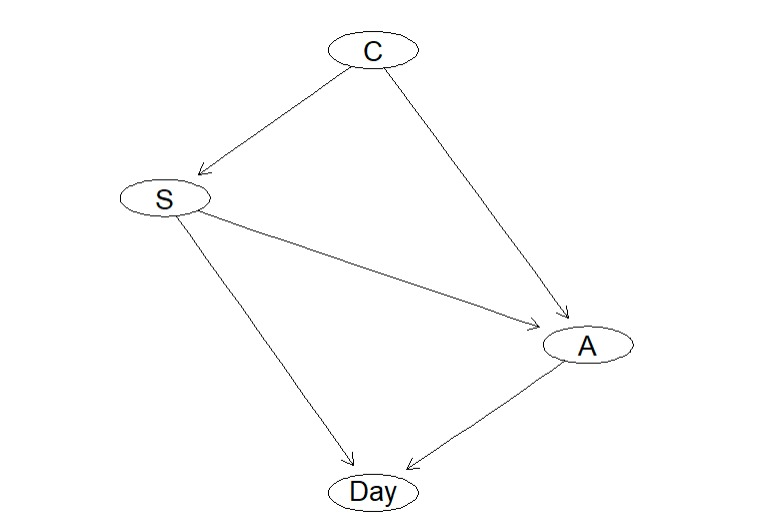
\includegraphics[width=0.55\textwidth]{img/dag3.jpeg}
\caption{DAG 3 - Red bayesiana para uso de transporte privado en mujeres de 60-80 años}
\label{fig:dag3}
\end{figure}

4.	Para nuestro ultimo escenario calculamos si los viajes en estratos bajos tienden a ser más largos en transporte público que en automóvil, como se puede analizar este caso es similar al caso dos en el sentido en que no nos pide calcular una probabilidad si no comparar dos medias por lo que seguimos el mismo procedimiento que con el caso dos y obtuvimos como resultado que en promedio duran mas los viajes en transporte publico dado que las personas pertenecen a un estrato bajo. La función utilizada fue la siguiente:

$$E(T \,|\, E = 1, M2 = transporte publico)$$
$$E(T \,|\, E = 1, M2 = auto)$$
$$T = (H - I) * 60 + (F - M)$$
Donde:\\
I = Hora de inicio\\
M = Minuto de inicio\\
H = Hora fin\\
F = Minuto Fin\\
E = estrato\\
M2 = Medio de transporte\\

\begin{figure}[h]
\centering
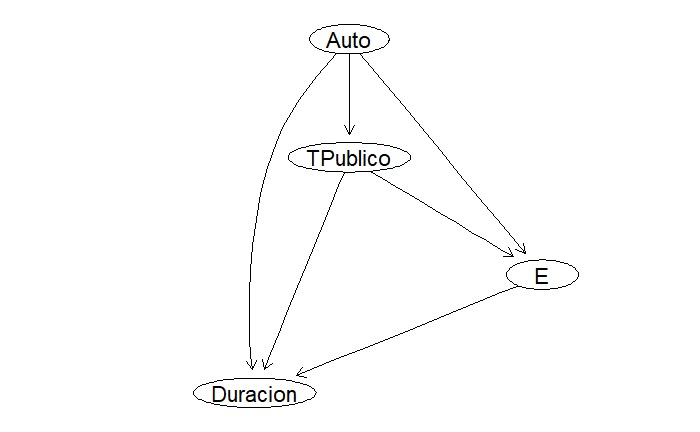
\includegraphics[width=0.5\textwidth]{img/dag4.jpeg}
\caption{DAG 4 - Red bayesiana para comparación de tiempos de viaje entre modos de transporte}
\label{fig:dag4}
\end{figure}

\section{Conclusiones}

Las redes bayesianas multinomiales, junto con el algoritmo Hill Climbing, fueron necesarias para modelar la movilidad urbana y sus desigualdades. Las consultas de las probabilidades mostraron diferencias en tiempos de viaje, gastos y usos de transporte según la edad, género y estrato socioeconómico. Estos resultados nos dieron a entender que los trayectos no solo tienen valor académico, sino también potencial para orientar políticas públicas de transporte más equitativas.

% Ejemplo de Referencias (Se puede usar .bib o manual)
\bibliographystyle{ieeetr}
\bibliography{referencias}

\end{document}